\section{Algorithm Perspective: Slow Alignment}
% The Absorption Rate Does Not Depend on the Training Set
\label{sec:algorithm}

Section~\ref{sec:data} analyzed the one-shot gain from the data side: what a query is worth to the student is set by the states its rollouts reach. Turning to the algorithm side, this section asks \textit{why one query keeps producing gains over so many steps}.

\begin{tcolorbox}[takeawaysbox]
\begin{itemize}[topsep=0pt, partopsep=0pt, leftmargin=12pt, itemsep=0pt]
    \item \textbf{Alignment slows over time, and this trend is insensitive to query count.} The student continuously narrows the teacher–student gap throughout the run, but the rate of progress diminishes steadily, which is why a run requires hundreds of steps rather than tens. Increasing the number of queries does not accelerate or decelerate this process.

    \item \textbf{Even a fixed set of states takes hundreds of steps to learn from.}
    A run that trains on the same states from beginning to end still improves over hundreds of steps, so a steady supply of fresh states is not required to keep a run going that long.
\end{itemize}
\end{tcolorbox}

\subsection{Alignment Metrics}
\label{sec:rate-setup}

OPD aligns the student with the teacher. Two quantities describe the state of that alignment at any moment: how much teacher--student disagreement is left, and how fast it is falling. We measure both on the states the student actually visits.

\begin{itemize}[topsep=2pt, partopsep=0pt, leftmargin=13pt, itemsep=2pt, parsep=0pt]
    \item \textbf{Distance.} The teacher and the student disagree at each visited position, by the per-token advantage of Eq.~\ref{eq:token-advantage}. We take the \emph{distance} \(d_t\) to be the average size of that disagreement over the positions \(\mathcal{T}_t\) the student visits at step \(t\):
    \begin{equation}
        d_t
        =
        \frac{1}{|\mathcal{T}_t|}
        \sum_{i\in\mathcal{T}_t}
        \left|
            \log\pi_T(y_i\mid s_i)-\log\pi_{\theta_t}(y_i\mid s_i)
        \right|.
        \label{eq:distance}
    \end{equation}
    Here \(s_i=(x,y_{<i})\) is the state at token position \(i\), as defined in Section~\ref{sec:prelim}. Averaging magnitudes keeps positive and negative per-token gaps from cancelling, so \(d_t\) falls to zero only as the two policies come to agree at the positions the student visits.
    \item \textbf{Absorption rate.} The \emph{absorption rate} \(v_t\) is then the proportion of that distance one update absorbs,
    \begin{equation}
        v_t = \frac{d_t-d_{t+1}}{d_t}.
        \label{eq:absorption-rate}
    \end{equation}
\end{itemize}
We track both metrics from step 30, after gradient clipping no longer binds. Since each run measures distance over the states it visits, these runs have settled at different levels by then. We therefore report each run against its own value at step 30, which we refer to as the \emph{distance left} \(d_t/d_{30}\).\footnote{Late in training a single pair of consecutive steps is too noisy to read, so \(v_t\) is estimated over the geometric window \([t/1.4,\,1.4t]\), which is why it stops short of step \(300\). Appendix~\ref{app:alignment-dynamics} gives the estimators and the evidence behind both conventions.}

\subsection{Alignment Slows Similarly Across Data}
\label{sec:mech-dynamics}

We track \(d_t\) and \(v_t\) for OPD trained on 1, 4, 16, and all DAPO-Math-17k queries, over the same \(300\) steps and under the mathematical configuration of Section~\ref{sec:setup}.

\begin{figure}[t]
    \centering
    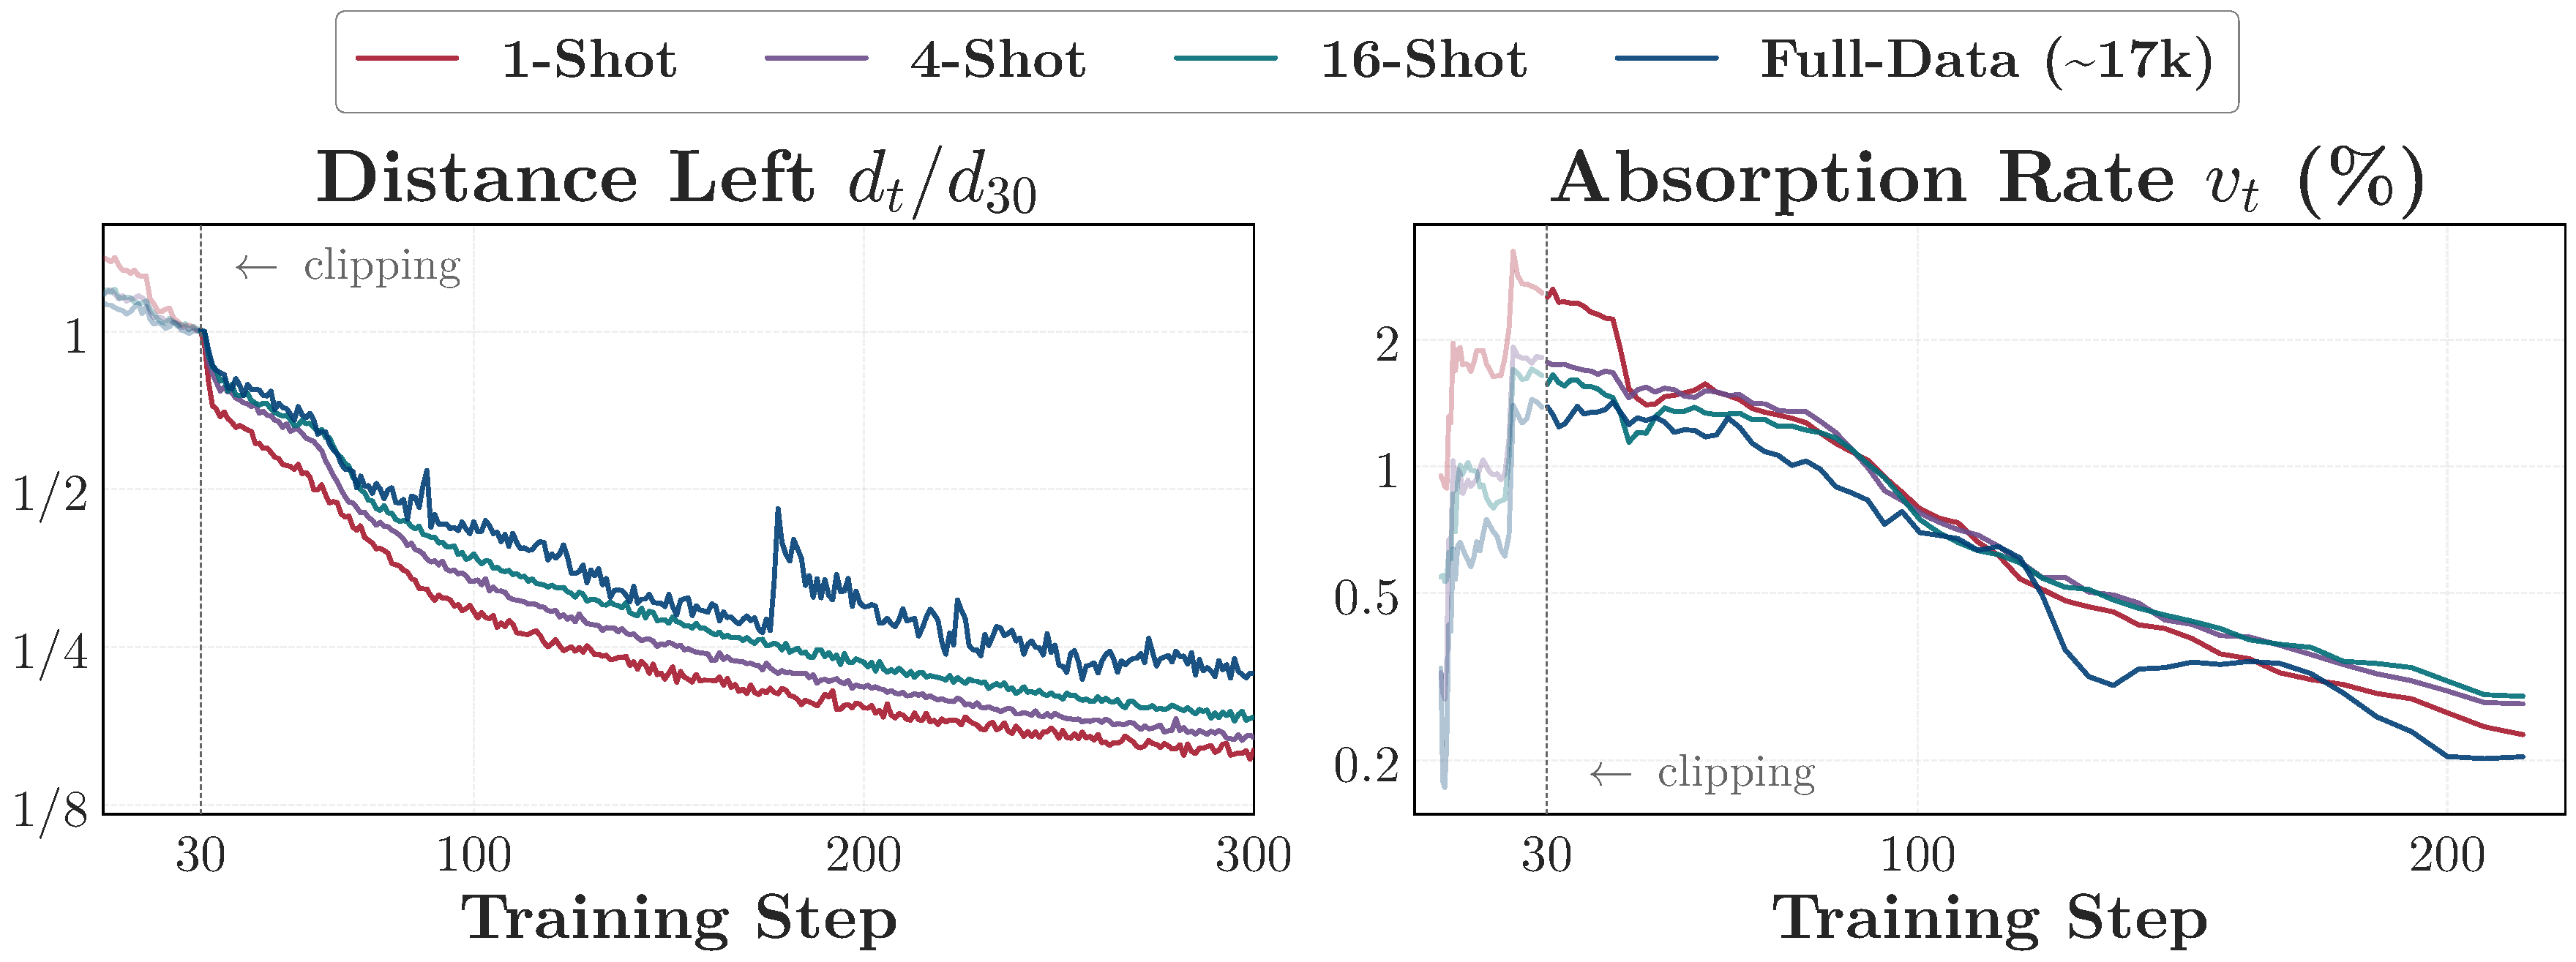
\includegraphics[width=0.75\linewidth]{figures/5_digestion_rate_v2.pdf}
    \caption{
    Teacher--student alignment for OPD trained on 1, 4, 16, and all DAPO-Math-17k queries. Distance (left) and absorption rate (right) are both on logarithmic vertical axes against linear steps.
    }
    \label{fig:alignment-contraction}
\end{figure}

\paragraph{The student aligns ever more slowly.}
The distance falls for the whole run, so the student is never stuck. What slows is the absorption rate, which falls throughout the run in the right panel of Figure~\ref{fig:alignment-contraction}: on the logarithmic distance axis at left a constant rate would trace a straight line, and all four curves bend flatter instead. Each update thus absorbs less of what is left than the last, which is why a run takes hundreds of steps rather than tens.

\paragraph{The absorption rate falls in much the same way at every training-set size.}
The four runs do this alike: each removes \(78\%\) to \(84\%\) of its step-\(30\) distance by step \(300\), and all four slow by a similar factor during training (Appendix~\ref{app:alignment-dynamics} gives the per-run numbers and the conventions these readings are taken under). One query therefore does not make alignment slower or faster: the pace is a property of OPD rather than of the training set. The learning rate changes how many steps that takes, but not the way the distance falls (Appendix~\ref{app:lr-sensitivity}).

\subsection{Ablation on Fixed States}
\label{sec:fixed-states}
On-policy training keeps producing new states as the student changes, and one reading of the hundreds of steps is that the run lasts as long as that supply does. Holding the training states fixed tests that reading directly: if a fixed set of states is exhausted quickly, the off-policy run should finish early.

\paragraph{Setup.}
We compare two one-shot runs that differ only in where their training states come from. The always-on-policy run draws fresh rollouts from the current student at every step. The always-off-policy run reuses the \(64\) trajectories of Section~\ref{sec:state-diversity}, sampled once from the initial student, for every update, so its training states stay fixed while the student changes.

\paragraph{Holding the states fixed leaves the run just as long.}

\begin{figure}[t]
    \centering
    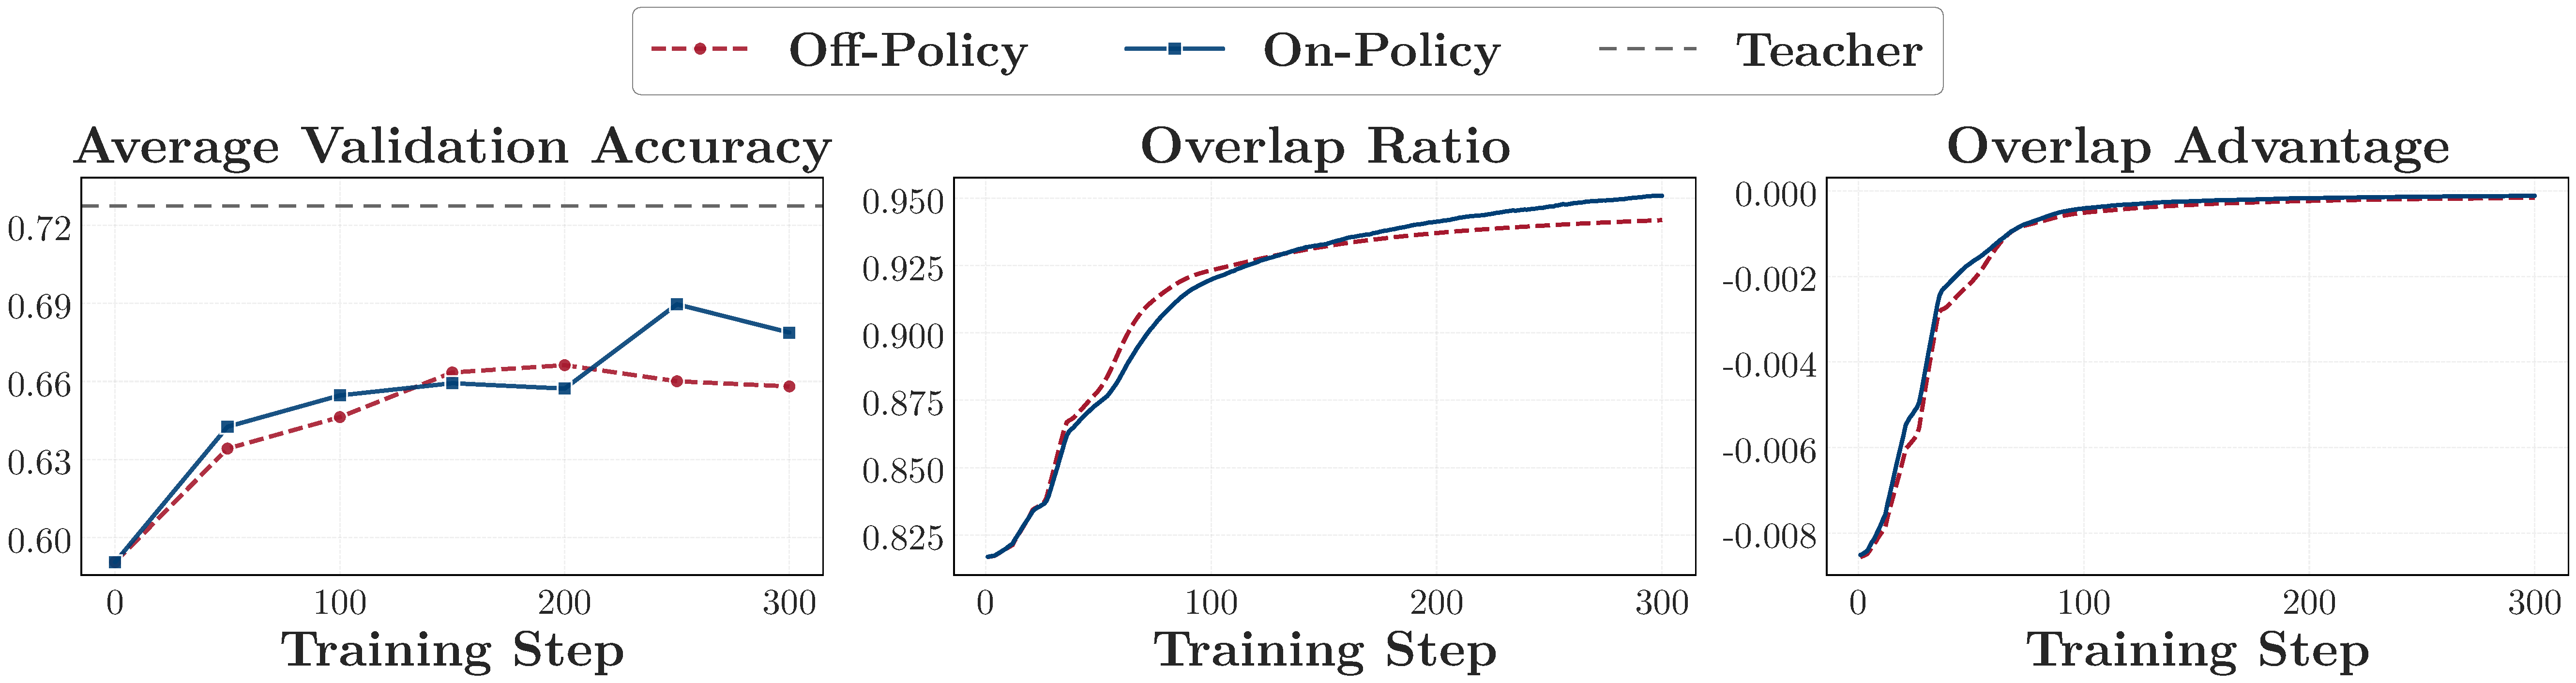
\includegraphics[width=\linewidth]{figures/5_online_offline.pdf}
    \caption{
    Validation accuracy and alignment metrics for the on-policy and off-policy one-shot runs.
    }
    \label{fig:online-offline}
\end{figure}
Figure~\ref{fig:online-offline} shows the off-policy run gains accuracy steadily for about \(200\) steps and then stops, so its gain builds up over hundreds of steps rather than over the first few updates. The alignment metrics move just as slowly: the off-policy run's top-\(16\) token overlap rises and its overlap-token advantage approaches zero only over hundreds of steps. Removing that supply therefore does not shorten the run. 
% The off-policy run is even slightly ahead at steps \(150\) and \(200\), and ends \(2.1\) points below on-policy training at step \(300\), across three benchmarks. Fresh states therefore buy a modest gain in final accuracy rather than a faster run. 
This suggests that a fixed set of states is enough on its own to keep an OPD run going for hundreds of steps, so the length of a run is not explained by how long fresh states keep arriving.

